\section{System description} \label{sec:sys-descr}
The purpose of this section is to give an overview of the system which the project is based on. It is not of great importance which specific turbine is the subject of examination with regards to exploring and dealing with the floating control problem. But the specifications of the turbine determines the model parameters. Therefore this section is first and foremost dedicated to outlining the turbine specification and secondly to define the software environment which the system is derived from and evaluated upon. 

\subsubsection{The Vestas V164-8.0}
The turbine examined in this project is the Vestas V164-8.0 (8 MW) which is a variable-speed-variable-pitch turbine with a permanent magnet generator, gearbox and full-scale converter.

The turbines operating ranges are:
\begin{itemize}
	\item Cut in: 4 m/s
	\item Nominal: 13 m/s
	\item Cut out: 25 m/s
	\item Survival: 50 m/s
\end{itemize}
The rotor diameter is 164 m and the hub height is 100 m. The nominal power output is 8 MW with the power curve seen in \cref{fig:v164_8mw_pc}
\begin{figure}[ht]
	\centering	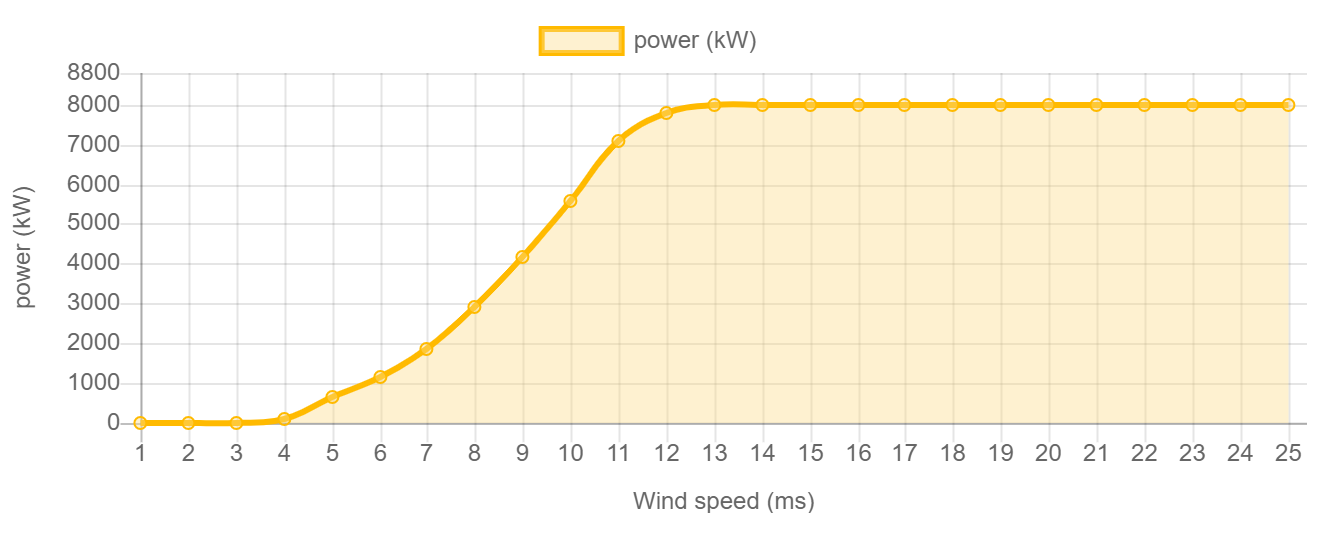
\includegraphics[width=0.95\linewidth]{Graphics/v164-8mw_powerCurve.PNG}
	\caption{The power curve of the Vestas V164-8MW Wind Turbine found at \cite{LucasBauer}}
	\label{fig:v164_8mw_pc}
\end{figure}

\subsubsection{Simulation environment}
It is deemed both unfeasible and unnecessary to test the controller derived in this project on an actual real world turbine. In stead it is tested in a realistic simulation environment and thus when referring to the \textit{real} system or turbine it is a reference to the simulated turbine. Vestas has a WT simulator called VTS which is a high-fidelity simulation tool used to simulate the behaviour and loads of specific Vestas WTs. The simulation tool has several outputs. One of them are time-series data from both simulated sensors and controller variables. The data is initially confined in files with a custom Vestas file format but can be extracted with a matlab tool. VTS enables the possibility of easily defining wind conditions and parameters for controllers. Furthermore through the use of Matlab Simulink controller structures can also be redefined. VTS does not natively support floating simulations but an extension with OrcaFlex enables it. VTS simulates turbine loads from the tower bottom and up while OrcaFlex simulates the foundation and its interaction with the waves. During simulations information is shared between VTS and OrcaFlex. OrcaFlex can be configured to simulate specific sea conditions.

Notable simulation environment changes used in parts of this project are:
\begin{itemize}
	\item Wind speeds are above 14 m/s to stay well inside the FLC region. It is considered outside the scope of this project to consider operation around nominal wind speed and in PLC.
	\item Turbulence is removed for some simulations such that the system response is easier to deduce and model. 
	\item The FATD controller is turned off such that there is no damping of the fore-aft motion.
	\item OrcaFlex is set up to simulate flat, still water to simplify the system response even further. 
\end{itemize}

